\chapter{Wstęp teoretyczny}
\label{teorethical_introduction}

\section{Zastosowane protokoły i systemy}
Zgodnie z założeniami pracy, aby zrealizować postawiony urządzeniu cel, zdecydowano się wykorzystać wymienione poniżej protokoły i interfejsy:
\begin{itemize}
	\item \textbf{GSM} - Wykorzystywany do komunikacji zdalnej dalekiego zasięgu (wysyłanie danych na serwer oraz komunikacja z użytkownikiem)
	\item \textbf{GPS} - Wykorzystywany do wyznaczenia lokalizacji pojazdu, a także jego prędkości oraz azymutu.
	
	\item \textbf{NMEA0183} - Jest to standard w jakim moduł GPS wysyła dane do mikrokontrolera
	\item \textbf{Bluetooth Low Energy} - Wykorzystywany do komunikacji bliskiego i średniego zasięgu (komunikacja z użytkownikiem oraz z urządzeniem deaktywującym)
	\item \textbf{NFC} - Wykorzystywany do komunikacji bardzo bliskiego zasięgu (do wysłania klucza szyfrującego do- oraz komendy deaktywującej od urządzenia deaktywującego)
\end{itemize}

Wszystkie z powyższych protokołów zostały pokrótce opisane, a następnie krótko zestawione w tym rozdziale.

\clearpage

\section{System GSM}
\label{GSM}

Poniższy podrozdział powstał na podstawie źródeł \cite{GSM}, \cite{GSM_tutorialspoint} oraz \cite{GSM_wiki}.\\

System GSM (\textit{ang. \textbf{G}lobal \textbf{S}ystem for \textbf{M}obile Communication}) jest obecnie najpowszechniej wykorzystywanym systemem służącym do komunikacji bezprzewodowej dalekiego zasięgu. System ten wykorzystywany jest do przesyłania głosu oraz serwisów danych. Pomysł na stworzenie sieci umożliwiającej komunikację głosową wyłonił się we wczesnych latach 70. ubiegłego wieku z opracowywanej w siedzibie Bell Laboratories mobilnej sieci radiowej. Jednakże dopiero dwanaście lat później, w 1982 roku powstał oficjalny komitet normalizacyjny nazwany \textit{Groupe Spécial Mobile}, którego zadaniem było utworzenie jednolitego, otwartego standardu dla telefonii komórkowej. 

Pierwotna wersja standardu działała w paśmie 900 MHz (880 - 960 MHz) i umożliwiała jedynie transmisję głosową. Jego kolejna wersja została opublikowana w 1990r. i definiowała ona dodatkowe pasmo 1800 MHz (1710 - 1880 MHz). Ponadto, umożliwiała przesyłanie krótkich wiadomości SMS (\textit{ang. \textbf{S}hort \textbf{M}essage \textbf{S}ystem}), a także faxu czy transmisję danych. Dalsze prace nad systemem wprowadziły do standardu techniki zwiększające przepustowość transmisji (maksymalna prędkość odbioru - 57.6 kb/s, maksymalna prędkość nadawania - 14.5 kb/s oraz 30 - 80 kb/s przy transmisji GPRS) oraz mechanizm przesyłania danych w pakietach GPRS (\textit{ang. \textbf{G}eneral \textbf{P}acket \textbf{R}adio \textbf{S}ervice}). 

Pomimo pojawienia się na świecie nowszych rozwiązań, takich jak sieci UMTS i LTE, ze względu na ogromną popularność, architektura sieci GSM wciąż jest rozwijana. 

System GSM umożliwia skorzystanie z następujących usług:
\begin{itemize}
	\item Połączenia głosowe - Stanowią one sztandarową funkcjonalność sieci GSM. Jej standard definiuje kodek GSM, który służy do zamiany głosu (skonwertowanego do napięciowego sygnału analogowego przez mikrofon) na postać cyfrową, która jest następnie kompresowana stratnie i transmitowana do odbiorcy. Stosowana jest kompresja na podstawie algorytmu LPC (ang. \textbf{L}inear \textbf{P}redictive \textbf{C}oding). Po stronie odbiorcy sygnał jest dekodowany, lecz ze względu na stratność LPC, słyszalny jest zniekształcony, nienaturalny głos rozmówcy.
	\item Transmisja danych - Umożliwia dostęp do internetu z urządzenia GSM, a także korzystanie z transmisji strumieniowej.
	\item Wiadomości tekstowe i multimedialne - Usługa przesyłania krótkich wiadomości tekstowych, o długości do 160 znaków, pod warunkiem korzystania jedynie z alfabetu łacińskiego. W przypadku stosowania znaków diakrytycznych maksymalny rozmiar wiadomości spada do 70 znaków. Wiadomości multimedialne (inaczej MMS), umożliwiają przesyłanie zdjęć, filmów czy dźwięków. Ich rozmiar maksymalny jest uzależniony od ograniczeń telefonu oraz operatora.
\end{itemize}

Jednym z głównych założeń systemu jest możliwość korzystania z niego przez wielu użytkowników jednocześnie. Aby rozwiązać ten problem, postanowiono zastosować technikę zmiany częstotliwości FDMA (\textit{ang. \textbf{F}requency \textbf{D}ivision \textbf{M}ultiple \textbf{A}ccess}) oraz okien czasowych TDMA (\textit{ang. \textbf{T}ime \textbf{D}ivision \textbf{M}ultiple \textbf{A}ccess}). Oznacza to, że pasmo częstotliwości GSM jest podzielone na wąskie kanały, o szerokości 200 kHz każdy. Czas użytkowania każdego kanału podzielony jest na 8 okien czasowych. Każde urządzenie ma zatem dostęp do sieci dostrajając się do odpowiedniego kanału w czasie trwania przydzielonego okna czasowego. Przedstawiono to na rysunku \ref{fig:image_gsm_frequencies_timeslots}.

\begin{figure}[H]
	\centering
	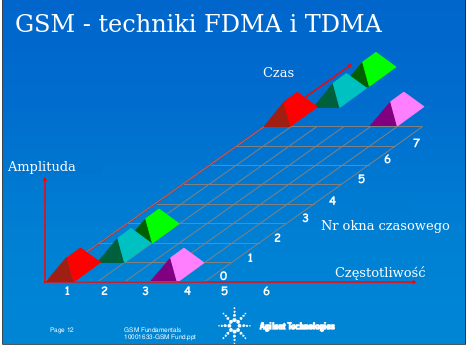
\includegraphics[width=8cm]{img/theory/GSM/gsm_timeslots_frequencies.png}
	\caption{Podział pasma częstotliwości na kanały i okna czasowe. Źródło: \cite{GSM}}
	\label{fig:image_gsm_frequencies_timeslots}
\end{figure}


Architektura sieci GSM powstała w oparciu o komórkowy system radiowy, skąd powszechnie stosowana nazwa - sieć komórkowa. Charakteryzuje się ona tym, że obszar terenu, na którym ma być prowadzona komunikacja radiowa dzieli się na tzw. komórki. Każdej komórce przypisana jest stacja bazowa (\textit{ang. \textbf{B}ase \textbf{T}ranceiver \textbf{S}tation}), która stanowi bramę dostępową do sieci. Urządzenie mobilne GSM, takie jak na przykład telefon, znajdując się na obszarze komórki najczęściej odbiera sygnał z więcej niż jednej stacji bazowej, jednakże zawiera połączenie z tą, której sygnał jest najsilniejszy. W razie spadku mocy sygnału stacji z którą urządzenie jest połączone, możliwa jest dynamiczna zmiana połączenia do innego BTS'a.

\begin{figure}[H]
	\centering
	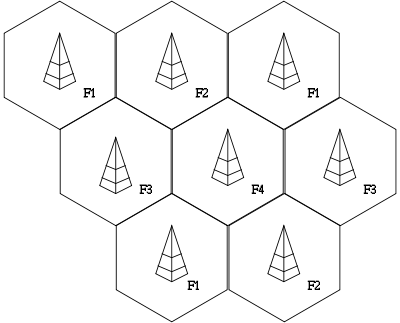
\includegraphics[width=8cm]{img/theory/GSM/cell_structure.png}
	\caption{Podział obszaru na komórki. Źródło: \cite{GSM_wiki}}
	\label{fig:image_gsm_cells}
\end{figure}

Aby móc korzystać z sieci GSM, urządzenia muszą posiadać kartę SIM (\textit{ang. \textbf{S}ubscriber \textbf{I}dentification \textbf{M}odule}). Oprócz przydatnych dla użytkownika wbudowanej pamięci na wiadomości SMS i kontakty, posiada unikalny na całym świecie numer identyfikujący użytkownika w sieci. W celu zalogowania się do sieci, urządzenie GSM musi podać ten numer w trakcie nawiązywania połączenia ze stacją bazową. 

Każda stacja bazowa wykorzystuje wiele kanałów GSM. Jednakże, aby nie dopuścić do wzajemnego zakłócania się, stacje bazowe z przylegających do siebie cel wykorzystują inne zbiory kanałów. Dodatkowo, w stacjach bazowych stosuje się dwa rodzaje anten - dookólne i kierunkowe o pokryciu 120\degree. Anteny dookólne pokrywają caly obszar komórki tym samym zbiorem kanałów, natomiast kierunkowe - dla każdego podobszaru wykorzystują ich inny zestaw. Ze względu na skończoną prędkość sygnału radiowego, istnieje również maksymalny promień pojedynczej komórki. W praktyce wynosi on około 35 km. Poniważ istnieje konieczność umożliwienia prowadzenia komunikacji na tak duży zasięg, standard ten nie należy do najbardziej energooszczędnych. W zależności od klasy urządzenia, minimalna moc nadawanego sygnału może wynosić od 1 do 20 mW, natomiast maksymalna nawet do 8 W. Urządzenia GSM mają możliwość dostosowywania mocy transmisji na podstawie mocy sygnału odebranego od stacji bazowej, w celu ograniczenia  wysokiego zużycia energii. 

Biorąc jednak pod uwagę fakt, iż transmisja przebiega w oknach czasowych, moc średnia jest niższa. Każde okno czasowe trwa 577 $\mu s$, a w jego czasie można wysłać jedną z kilku ramek komunikacyjnych. W trakcie każdej z nich można wysłać 148 bitów danych. W przypadku ramki nadawanej w trakcie rozmowy, głos kodowany jest jedynie na 57 bitach. Każde z urządzeń w sieci otrzymuje okno czasowe co 4.615 ms, liczone od początku okna, do rozpoczęcia następnego. Stąd wynika, że  w trakcie nadawania, urządzenie transmituje dane jedynie przez 12.5\% czasu. Pobór prądu, w zależności od odległości do nadajnika, a więc od mocy nadawania, może wówczas wynosić nawet do 1.5 A. Przyjmując napięcie zasilania układu GSM wynoszące 4 V, maksymalna pobierana moc średnia może wynosić:

\begin{gather}
 	P_{\text{śr}} = U \cdot I \cdot \tau \\
 	P_{\text{śr}} = 4 V \cdot 1.5 A \cdot 0.125 = 0.75 W \nonumber 	
 	\label{eq_gsm_power_mean} 
\end{gather}
 gdzie:
 
 $P_{\text{śr}} $ - moc średnia
 
 $U$ - napięcie zasilania układu,
 
 $I$ - nateżęnie prądu w momencie transmisji
 
 $\tau$ - współczynnik wypełnienia impulsu (czas trwania okna czasowego podzielony przez czas pomiędzy oknami czasowymi)
 
Wartość mocy średniej wynosząca 0.75 W odpowiada ciągłemu zużyciu prądu rzędu 187.5 mA przy napięciu zasilania układu rzędu 4 V. 




\section{System GPS}
\label{GPS}

Poniższy podrozdział powstał na podstawie źródeł \cite{GPS_ublox} oraz \cite{inzynierka}.\\



System GPS(\textit{ang. \textbf{G}lobal \textbf{P}ositioning \textbf{S}ystem}) był historycznie pierwszym systemem nawizgacji satelitarnej GNSS (\textit{ang. \textbf{G}lobal \textbf{N}avigation \textbf{S}attelite \textbf{S}ystem}). Powstał w wyniku prac w Departamencie Obrony Stanów Zjednoczonych i jest w pełni własnością rządu tego kraju. Oprócz niego istnieją jeszcze rosyjski GLONASS, a od niedawna europejski Galileo oraz chiński Beidou. Ostatnie dwa systemy satelitarne nie są jeszcze w pełni funkcjonalne, stanowią raczej systemy o zasięgu regionalnym niż globalnym.

Głównym elementem składowym systemów nawigacji satelitarnej, są jak sama nazwa wsazuje satelity. Poruszają się one po ściśle określonych, stałych orbitach, które są tak dobrane, aby z dowolnego punktu na globie, w dowolnym momencie była możliwość odebrania sygnału z co najmniej czterech z nich. Przedstawia to rysunek \ref{fig:image_gps_basics}.

\begin{figure}[H]
	\centering
	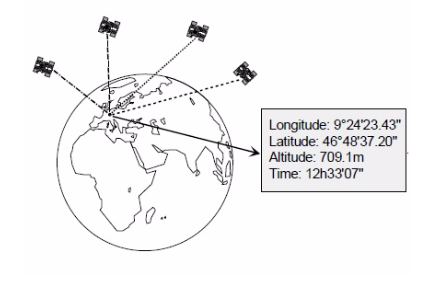
\includegraphics[width=10cm]{img/theory/GPS/gps_introduction.png}
	\caption{Model działania systemu GPS. Źródło: \cite{GPS_ublox}}
	\label{fig:image_gps_basics}
\end{figure}

Podstawę w systemach GNSS stanowi czas. Każdy z satelitów posiada 4 zegary atomowe, które stanowią najdokładniejsze źródło czasu znane ludzkości. Zegary te posiadają błąd rzędu 1 sekundy po upływie najwcześniej 30000 lat. Dodatkowo, są one co pewien czas synchronizowane ze źródłami na Ziemi.

Zadaniem każdego z satelitów jest nadawanie w formie rozgłoszeniowej sygnału, w którym zawarta jest wiadomość o jego lokalizacji na orbicie oraz czasie w momencie wysyłania wiadomości. Sygnał ten nadawany jest drogą radiową więc jego prędkość jest równa prędkości światła. Po dotarciu do odbiornika jest on bardzo słaby, przez co praktycznie niemożliwe jest jego odebranie wewnątrz budynków, a w pobliżu wysokich obiektów dokładność lokalizacji spada. Najdokładniejsze wyniki wyznaczania pozycji można osiągnąć na otwartej przestrzeni. Podstawowy sygnał przesyłany jest na fali nośnej o częstotliwości 1575.42 MHz i nosi nazwę L1.

Ponadto, sygnał GPS (a także pochodzący z innych systemów lokalizacji satelitarnej) ulega łatwo zakłóceniom w momencie przejścia przez jonosferę, bowiem fala elektromagnetyczna ulega na niej załamaniu, przez co zmienia swój tor i wydłuża drogę. W efekcie, pomiary odległości od odbiornika do satelity, niezbędne do wyznaczenia lokalizacji przestają być dokładne i pojawia się błąd lokalizacji.
Problem ten rozwiązano na 2 sposoby. Pierwszym z nich jest nadawanie sygnału przez satelity na kilku częstotliwościach. Każda z nich, przechodząc przez jonosferę ulega załamaniu, lecz pod innym kątem, przez co pokonają różne długości drogi przebytej do odbiornika, a tym samym zostaną odebrane w różnych momentach. Dzięki temu, odbiornik jest w stanie wyznaczyć korektę i wyeliminować błąd. Pierwotnie, rozwiązanie to było dostępne jedynie w celach militarnych, lecz od 2005 roku, Departament Obrony Stanów Zjednoczonych udostępnił częstotliwość L2 (1227.60 MHz) do celów cywilnych, a od 2008r. - również L5 (1176.45 MHz). Częstotliwości dostępne w systemie GPS pokazano na rysunku \ref{fig:image_gps_frequencies}.

\begin{figure}[H]
	\centering
	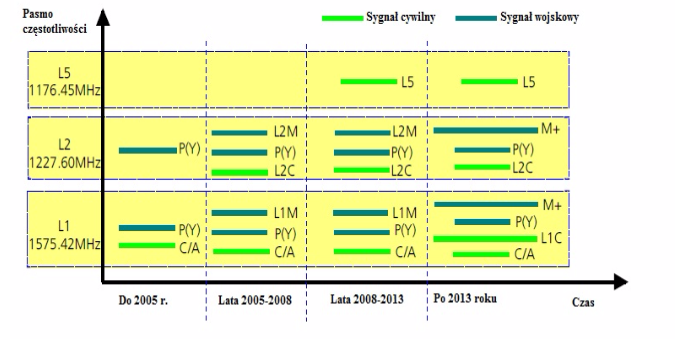
\includegraphics[width=15cm]{img/theory/GPS/gps_frequencies.png}
	\caption{Zbiór częstotliwości wykorzystywanych w systemie GPS. Źródło: \cite{inzynierka}}
	\label{fig:image_gps_frequencies}
\end{figure}

Druga metoda to wyznaczenie korekty dla przejścia przez jonosferę w stacjach naziemnych, a następnie rozgłaszanie depeszy ją zawierającej poprzez sieć stacji bazowych. Rozwiązanie to nosi miano DGPS (\textit{ang. \textbf{D}ifferential \textbf{GPS}}). Dzięki zastosowaniu tej techniki, dokładność lokalizacji wzrasta z nominalnych 15 m nawet do 10 cm.

Układy GPS, które umożliwiają skorzystanie z któregoś z tych dwóch rozwiązań są jednak kosztowne, więc na rynku cywilnym najpowszechniej stosowane są moduły wykorzysujące jedynie częstotliwość L1. Dzięki temu, za kilkadziesiąt złotych można uzyskać system z dokładnością do kilku metrów w sprzyjających warunkach \cite{inzynierka} (Rozdział 7 - Testy urządzenia). W pracy tej uzyskano dokładność systemu rzędu 1 - 2 metrów przy braku zakłóceń, oraz 5 - 7 metrów idąc wzdłuż wysokich budynków.

Aby zrozumieć zasadę działania systemu GPS proszę wyobrazić sobie sytuację jak na rysunku \ref{fig:image_gps_basics1}:

\begin{figure}[H]
	\centering
	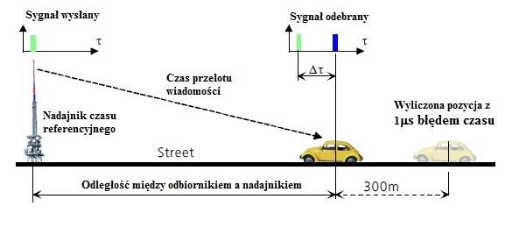
\includegraphics[width=12cm]{img/theory/GPS/gps_basics1.png}
	\caption{Zasada działania systemu GPS. Źródło: \cite{inzynierka}}
	\label{fig:image_gps_basics1}
\end{figure}

Załóżmy, że w przedstawionym pojeździe znajduje się odbiornik GPS. W pewnym momencie odbiera on sygnał GPS z nadajnika referencyjnego. W sygnale znajduje się wartość czasu w momencie wysłania wiadomości. Ze względu na skończoną prędkość światła ($c = 299 792 458 m/s$), zostanie ona odebrana przez odbiornik z pewnym opóźnieniem. Wykorzystując ten fakt i znając prędkość transmisji (wartość prędkości światła), można wyznaczyć odległość do nadajnika:

\begin{equation}
	D = c \cdot \Delta t
\end{equation}

gdzie,

$D$ - odległość między nadajnikiem i odbiornikiem

$c$ - prędkość światła

$\Delta t$ - różnica czasu między wysłaniem i odebraniem wiadomości

Aby wyznaczyć różnicę czasu, odbiornik powinien mieć również własny zegar. Powinien on być przy tym niezwykle dokładny i zsynchronizowany z zegarem w nadajniku, bowiem błąd rzędu 1 $\mu s$ powoduje błąd lokalizacji rzędu 300 m. Ponieważ uzyskanie takiej dokładności oraz synchronizacji w każdym odbiorniku jest niemożliwe, należało znaleźć sposób umożliwiający rezygnację z konieczności posiadania zegara w odbiorniku. Przedstawiono go na rysunku \ref{fig:image_gps_basics2}:

\begin{figure}[H]
	\centering
	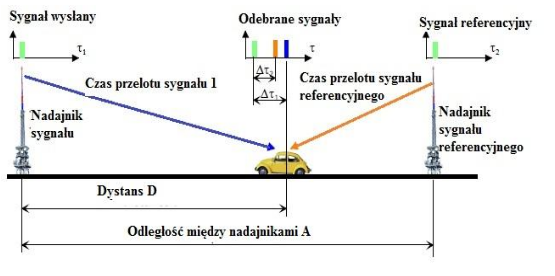
\includegraphics[width=12cm]{img/theory/GPS/gps_basics2.png}
	\caption{Zasada działania systemu GPS - sygnał referencyjny. Źródło: \cite{inzynierka}}
	\label{fig:image_gps_basics2}
\end{figure}

Polega on na zastosowaniu dodatkowego sygnału referencyjnego czasu. Wówczas po odebraniu obu sygnałów (które zostały wysłane w tym samym momencie) otrzymujemy:

\begin{equation}
\begin{cases}
\Delta \tau_1 \cdot c = D \\ 
\Delta \tau_2 \cdot c = A - D
\end{cases}
\end{equation}

Gdzie:

$\tau_1$ - różnica czasu między wysłaniem sygnału z nadajnika, a momentem jego odebrania

$\tau_2$ - różnica czasu między wysłaniem sygnału z nadajnika referencyjnego, a momentem jego odebrania

$A$ - odległość między nadajnikami

$D$ - odległość od nadajnika do odbiornika\\

Po odjęciu od pierwszego równania drugiego otrzymamy:

\begin{gather}
(\Delta \tau_1  - \Delta \tau_1) \cdot c = 2D - A \\
D = \frac{(\Delta \tau_1  - \Delta \tau_1) \cdot c + A}{2} \nonumber 
\end{gather}

Ponieważ jednak:

\begin{equation}
\begin{cases}
	\Delta \tau_1 = t - \tau_1 \\
	\Delta \tau_2 = t- \tau_2
\end{cases}
\end{equation}

to

\begin{equation}
(\Delta \tau_1 - \Delta \tau_2) = ((t - \tau_1) - (t - \tau_2)) = \tau_2 - \tau_1
\end{equation}

Gdzie:

$t$ - czas w momencie nadania sygnału przez nadajniki

$\tau_1$ - różnica czasu między wysłaniem sygnału z nadajnika, a momentem jego odebrania

$\tau_2$ - różnica czasu między wysłaniem sygnału z nadajnika referencyjnego, a momentem jego odebrania

Powyższe równania prowadzą do wniosku, że zastosowanie dodatkowego nadajnika referencyjnego, zsynchronizowanego z satelitami powoduje eliminację konieczności posiadania zegara w odbiorniku.

W rzeczywistości, takim nadajnikiem referencyjnym jest inny satelita GPS, bowiem są one ze sobą zsynchronizowane i nadają w dokładnie tym samym momencie.

Wyznaczona powyżej odległość $D$ dotyczy odcinka (jednej współrzędnej), a w rzeczywistości do wyznaczenia lokalizacji, uwzględniając satelitę referencyjnego, potrzeba sygnału z co najmniej 4 satelitów.



\section{Protokół NMEA 0183}
\label{NMEA}

Niniejszy podrozdział powstał na podstawie źrodeł \cite{inzynierka} oraz \cite{QUECTEL_HW_DESIGN}.\\

Protokół ten stanowi standard komunikacji między urządzeniami elektronicznymi wykorzystywanymi w urządzeniach morskich, zwłaszcza urządzeniami do lokalizacji i nawigacji. Zawiera on specyfikację elektryczną oraz opis ramek (wiadomości) wymienianych między modułami. Powstał w Stanach Zjednoczonych w \textit{\textbf{N}ational \textbf{M}arine \textbf{E}lectronics \textbf{A}ssociation}. Jego najnowsza, czwarta wersja pochodzi z listopada 2008 roku. 
Protokół ten pierwotnie wykorzystywał interfejs RS232, lecz w wersji drugiej dokonano jego zmiany na RS422. Interfejsy te różnią się jedynie poziomami napięć przypisanym logicznym wartościom bitów 0 i 1. 
Oba z nich umożliwiają wysyłanie danych bajt po bajcie. Każdy z nich rozpoczyna się bitem START (stan niski w RS422), który umożliwia odbiornikowi wykrycie początku bajtu i synchronizację. Następnie wysłanych jest kolejno 8 bitów danych, po których przesyłany jest bit parzystości (0 gdy liczba bitów w bajcie danych o wartości 1 jest parzysta lub 1 gdy jest nieparzysta) i na koniec - bit stopu. Przedstawiono to na rysunku \ref{fig:image_nmea_rs422}.

\begin{figure}[H]
	\centering
	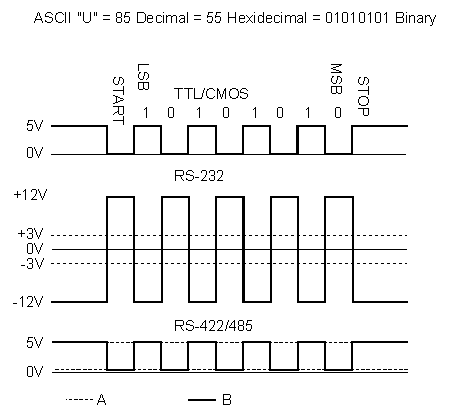
\includegraphics[width=10cm]{img/theory/NMEA/RS232_RS422.png}
	\caption{Poziomy napięć i kolejnośc bitów w interfejsach RS232 i RS422. Źródło: \cite{RS422}}
	\label{fig:image_nmea_rs422}
\end{figure}

Na podstawie tego interfejsu, NMEA nabudowała wyższą warstwę protokołu w postaci wiadomości. Każda wiadomość rozpoczyna się symbolem '\textbf{$\$$}', po którym występuje 2 literowy kod mówiący o type urządzenia (GP - urządzenie GPS, GN - urządzenie GLONASS) i 3 literowy kod definiujący typ przesyłanej wiadomości. Po kodzie występuje przecinek, a następnie lista pól danych oddzielonych przecinkami. W obrębie wiadomości, każde pole ma ściśle określoną funkcję i w razie nie występowania, musi zostać przesłane jako puste. Za ostatnim polem występuje znak '\textbf{*}', po którym znajduje się suma kontrolna, liczona jako funkcja Exclusive Or (XOR) ze wszystkich znaków między '\textbf{$\$$}', a '\textbf{*}' bez ich uwzględnienia. 

Lista zdefiniowanych wiadomości jest bardzo długa, jednak w tabeli \ref{table:table_nmea_messages} zestawiono najpowszechniej wykorzystywane w odbiornikach GPS.

\begin{table}[H]
\centering
\caption{Najczęściej wykorzystywane wiadomości NMEA0183 w odbiornikach GPS.\\ Źródło: \cite{inzynierka}}
\label{table:table_nmea_messages}
\begin{tabular}{| l | l |}
\hline
GGA & Najczęściej wykorzystywane dane związane z ustalaniem pozycji GPS \\  \hline
GGL & Pozycja geograficzna – długość, szerokość \\  \hline
GSA & Informacje o aktywnych satelitach oraz o jakości połączenia \\ 
    & (DOP – \textit{ang.    Dilution of Position}) \\ \hline
GSV & Informacje o satelitach w zasięgu \\ \hline
RMC & Rekomandowane minimum danych GNSS \\ \hline
VTG & Dane o kursie oraz prędkości \\ \hline
ZDA & Wiadomość z aktualnym czasem i datą \\ \hline
\end{tabular}
\end{table}

W niniejszej pracy, aby zrealizować założenia projektu niezbędne było sparsowanie (przeanalizowanie) danych z dwóch wiadomości nadawanych przez moduł GPS: GGA i VTG.
Z wiadomości GGA  wyłoniono informacje o długości i szerokości geograficznej, wskaźnikach półkul, statusie wyznaczenia lokalizacji, jakości odebranego sygnału, liczbie satelitów w zasięgu oraz wysokości nad poziomem morza. Wiadomość VTG została wykorzystana w celu uzyskania informacji o kursie (azymucie) oraz prędkości odbiornika. Ich struktury przedstawiono kolejno w tabelach \ref{table:table_nmea_gga_message} i \ref{table:table_nmea_vtg_message}.

\begin{table}[H]
\centering
\caption{Struktura wiadomości GGA. Źródło: Twórczość własna}
\label{table:table_nmea_gga_message}
\begin{tabular}{| l | l |}
\hline
\textbf{Pole} & \textbf{Opis} \\ \hline
\$ & Symbol początku wiadomości  \\ \hline
GP & Typ urządzenia  \\ \hline
GGA & Typ wiadomości  \\ \hline
130305.743 & Czas UTC w formacie hhmmss.sss \\ \hline
4717.115 & Szerokość geograficzna w formacie ddmm.mmm \\ \hline
N & Wskaźnik półkuli (N - północna, S - południowa) \\ \hline
00833.912 & Długość geograficzna w formacie dddmm.mmm  \\ \hline
E & Wskaźnik półkuli (W - zachodnia, E - wschodnia) \\ \hline
1 & Wskaźnik informujący o statusie wyznaczania pozycji \\ 
 & 0 - pozycja nieustalona \\ 
 & 1 - pozycja ustalona na podstawie sygnału z satelitów \\ 
 & 2 - pozycja ustalona przy pomocy DGPS \\ 
 & 6 - pozycja wyestymowana za pomocą mechanizmu \textit{Dead reckoning} \\ \hline
08 & Liczba satelitów z których odebrano sygnał \\ \hline
0.94 & Wskaźnik jakości sygnału (0.5 - najlepsza, 20 - bardzo niska) \\ \hline
00499 & Wysokość nad poziomem morza \\ \hline
M & Jednostki wysokości (M - metry) \\ \hline
047 & Różnica w wysokości między geoidą (Ziemią), a elipsoidą (przybliżeniem Ziemi) \\ \hline
M & Jednostki wysokości (M - metry) \\ \hline
,, & Dane DGPS (pole puste) \\ \hline
0000 & Numer identyfikacyjny stacji bazowej DGPS \\ \hline
* & Znak końca danych \\ \hline
58 & Suma kontrolna \\ \hline
$<$CR$><$LF$>$ & Znak końca wiadomości \\ \hline
\end{tabular}
\end{table}

\begin{table}[H]
\centering
\caption{Struktura wiadomości VTG. Źródło: Twórczość własna}
\label{table:table_nmea_vtg_message}
\begin{tabular}{| l | l |}
\hline
\textbf{Pole} & \textbf{Opis} \\ \hline
\$ & Symbol początku wiadomości  \\ \hline
GP & Typ urządzenia  \\ \hline
VTG & Typ wiadomości  \\ \hline
227.15 & Kurs (azymut) w stopniach \\ \hline
T & Pole stałe, zawierające symbol T \\ \hline
,, & Kurs magnetyczny (nie zaimplementowany przez producenta) \\ \hline
M & Pole stałe, zawierające symbol M \\ \hline
0.00 & Prędkość \\ \hline
N & Pole stałe opisujące jednostki prędkości (N - węzły, K - kilometry na godzinę) \\ \hline
0.00 & Prędkość \\ \hline
K & Pole stałe opisujące jednostki prędkości (N - węzły, K - kilometry na godzinę) \\ \hline
A & Tryb pozycjonowania \\
  & N - brak pozycji \\
  & A - pozycja na podstawie sygnału z satelitów \\
  & D - pozycja na podstawie DGPS \\ \hline
* & Znak końca danych \\ \hline
3E & Suma kontrolna \\ \hline
$<$CR$><$LF$>$ & Znak końca wiadomości \\ \hline
\end{tabular}
\end{table}



\section{Protokół Bluetooth Low Energy}
\label{bluetooth}

Poniższy podrozdział powstał na podstawie źródeł \cite{BLE} oraz \cite{inzynierka}.\\

Projekt protokołu BLE (\textit{ang. \textbf{B}luetooth \textbf{L}ow \textbf{E}nergy}) został zapoczątkowany przez firmę Wibree należącą do grupy Nokia. Celem nadrzędnym, który przyświecał jego autorom nie było utworzenie kolejnego protokołu, którego zastosowanie byłoby przesadnie szerokie. Zamiast tego, zdecydowali się oni na zaprojektowanie standardu radiowego umożliwiającego najniższe możliwe zużycie energii, a przy tym nieskomplikowanego, przez co możliwe byłoby zastosowanie go w systemach o niskich kosztach budowy. Innymi słowy są to założenia idealne dla rynku smartfonów oraz IoT (\textit{ang. \textbf{I}nternet \textbf{o}f \textbf{T}hings}), gdzie urzadzenia zasilane są z niewielkich baterii (często CR2032). Dla przykładu, zakup w liczbie 1000 sztuk mikrokontrolera użytego w tej pracy - nRF52832 wyprodukowanego przez Nordic Semiconductor, który posiada wbudowany stos BLE, kosztuje jedynie 9.78 zł za sztukę.

W trakcie prac, projekt zostął przejęty przez grupę Bluetooth SIG (\textit{ang. \textbf{B}luetooth \textbf{S}pecial \textbf{I}nterests \textbf{G}roup}), zrzeszającą dziesiątki firm i organizacji z wielu dziedzin przemysłu, zainteresowanych wykorzystywaniem i rozwojem protokołu Bluetooth. W roku 2010, Bluetooth Low Energy, znany również jako Bluetooth Smart został włączony do standardu Bluetooth 4.0, obok klasycznego protokołu Bluetooth Classic. Nie należy jednakże mylić tych dwóch protokołów komunikacyjnych, ponieważ poza warstwą fizyczną (interfejs radiowy o częstotliwości 2.4 GHz w pasmie ISM) różnią się w swych założeniach. Bluetooth Classic jest bowiem typowym protokołem umożliwiającym szybką, lecz energochłonną komunikację. W grudniu 2013 roku wprowadzono pierwszą dużą poprawkę do protokołu (Bluetooth 4.1), a rok później dalsze modyfikacje w postaci standardu Bluetooth 4.2. 

Bluetooth Low Energy, ze względu na swoje założenie o onergoszczędności posiada pewne ograniczenia. Pierwszym z nich jest przepustowość danych. Górna granica prędkości transmisji wynosi 1 Mb/s, jednakże jest to wartość jedynie teoretyczna. W praktyce jest ona obwarowana wieloma ograniczeniami sprzętowymi producentów mikrokontrolerów. W standardzie zawarte jest, iż pojedynczy pakiet danych może zawierać maksymalnie 20 bajtów. Ograniczenie sprzętowe wynika tu z częstotliwości wysyłania pakietów. Dla  mikrokontrolera Nordic Semiconductor z rodziny nRF51, wynosi ona do 6 pakietów na każdy interwał połączenia. Jest to konfigurowalny parametr, określający odcinek czasu w obrębie którego jeśli nie dojdzie do transmisji pakietu, połączenie zostanie uznane za zerwane. Interwał połączenia może wynosić od 7.5 ms do 4 s. Przy założeniu najkrótszej wartości tego parametru otrzymujemy przepustowość:

\begin{equation}
	\text{Przepustowość} = 6 \text{pakietów/interwał} \cdot \frac{1000ms}{7.5ms} \cdot 20 \text{bajtów} = 15960 \text{bajtów/s} \approx 128 kb/s
\end{equation}

Jak widać jest to wartość znacznie odbiegająca od 1 Mb/s, jednakże w porównaniu do zysku na zużyciu energii jest to i tak bardzo dobry wynik. 

Kolejne ograniczenie to zasięg komunikacji. Oficjalnie, Bluetooth Low Energy posiada zasięg rzędu 50 m. Jest to jednak wartość trudna do uzyskania, silnie zależna od otoczenia (między urządzeniami nie może być przeszkód), mocą transmisji (rekonfigurowalna, im mniejsza tym zasięg mniejszy) oraz liczbą innych urządzeń znajdujących się w pobliżu, która to decyduje o zajętości kanałów. Pasmo częstotliwości (od 2.402 GHz do 2.480 GHz) wykorzystywanej przez protokół podzielone jest bowiem na 40 kanałów. Przedstawiono to na rysunku \ref{fig:image_ble_channels}.

\begin{figure}[H]
	\centering
	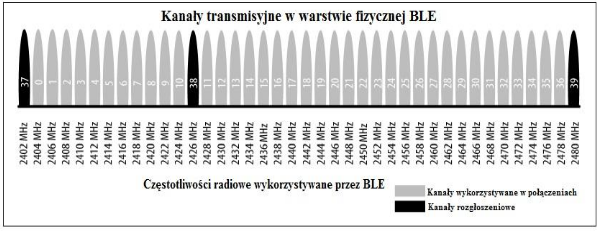
\includegraphics[width=17cm]{img/theory/BLE/ble_channels.png}
	\caption{Struktura pasma 2.4 ISM wykorzystywanego przez Bluetooth Low Energy.\\Źródło: \cite{inzynierka}}
	\label{fig:image_ble_channels}
\end{figure}

Protokół Bluetooth Low Energy oferuje dwie możliwości wysyłania danych. Pierwszym z nich jest bezpołączeniowe rozgłaszanie (\textit{ang. Advertising}). Wówczas, każde z urządzeń wysyła cyklicznie  w eter pakiet danych o pojemności do 31 bajtów. Interwał między pakietami może wynosić od 20 ms do 10.24 s. Jest to jednak komunikacja jednokierunkowa. Wysłane w ten sposób dane może odebrać każde urządzenie będące w zasięgu.

\begin{figure}[H]
	\centering
	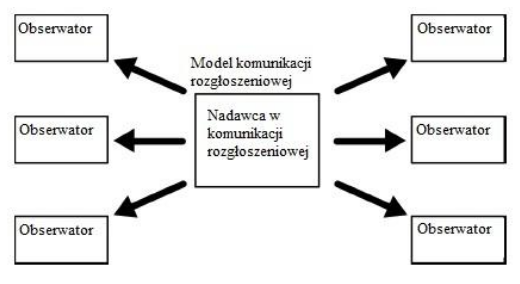
\includegraphics[width=12cm]{img/theory/BLE/ble_advertising.png}
	\caption{Model komunikacji rozgłoszeniowej. Źródło: \cite{inzynierka}}
	\label{fig:image_ble_advertising}
\end{figure}

Drugą metodą jest wysyłanie danych będąc w połączeniu. Wówczas komunikacja może być obustronna. W tym przypadku, BLE definiuje dwa możliwe typy urządzeń. Jedno z nich, które inicjuje połączenie określane jest jako \textit{Central}, natomiast urządzenie akceptujące połączenie - \textit{Peripheral}. Nie występuje przy tym ograniczenie, że urządzenie może mieć tylko jedną rolę. Może ono będąc w połączeniu urządzeniem typu \textit{Peripheral} zainicjować samodzielnie połączenie z innym odbiornikiem, a więc stać się dla tego połączenia\textit{Central'em}. Ważne jest, że urządzenie posiada jedną rolę dla danego połączenia, które jest realizowane typu punkt - punkt. 

Standard Bluetooth Low Energy definiuje logiczny podział struktur danych. Główną jednostką są tak zwane serwisy. Są to zgrupowania pewnych funkcjonalności, zwanych charakterystykami. Charakterystyki stanowią podstawowe jednostki komunikacji. Mogą one zawierać tzw. deskryptory, które są krótkimi, zrozumiałymi dla ludzi informacjami jak na przykład nazwa charakterystyki. Można to porównać do definicji klasy (serwis), zawierającej definicje metod (charakterystyk). Struktura ta zarzadzana jest przez tak zwany serwer GATT (\textit{ang. \textbf{G}eneric \textbf{Att}ribute Server}). Przedstawiono to na rysunku \ref{fig:image_ble_services}. 

\begin{figure}[H]
	\centering
	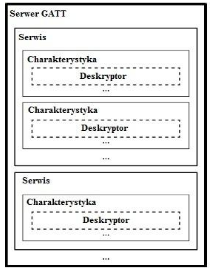
\includegraphics[width=5cm]{img/theory/BLE/ble_services.png}
	\caption{Model struktury danych serwera GATT. Źródło: \cite{inzynierka}}
	\label{fig:image_ble_services}
\end{figure}

Dla charakterystyk zostały zdefiniowane 4 metody komunikacji. Pierwsza z nich - \textit{Write}, polega na wysłaniu danych z urządzenia typu \textit{Central} do \textit{Peripheral}. Druga - \textit{Read}, umożliwia inicjatorowi połączenia odczytanie danych z urządzenia podległego. Pozostałe 2 metody - \textit{Notify} oraz \textit{Indicate} polegają na wysłaniu danych z urządzenia typu \textit{Peripheral} do urządzenia typu \textit{Central} lub odwrotnie, bez żadnego rządania transmisji ze strony odbiorcy. Różnica polega na tym, że \textit{Indicate} wymaga od odbiorcy wysłania potwierdzenia odbioru, a \textit{Notify} nie.



\section{Interfejs NFC}
\label{NFC}

Poniższy rozdział powstał na podstawie źródeł \cite{NFC} i \cite{NFC_NXP}.\\

Near Field Communication to protokół radiowy, stanowiący rozszerzenie swego starszego brata - interfejsu RFID. Mimo, iż jest do niego bardzo podobny w wielu aspektach, różni się znacznie pod względem założeń. RFID (\textit{ang. \textbf{R}adio \textbf{F}requency \textbf{Id}entification}), nie stanowi prawdziwego protokołu komunikacyjnego, bowiem pozwala jedynię na wymianę bardzo krótkich informacji, zwanych identyfikatorami. Urządzenia RFID stanowią bardzo proste układy. Składają się one zazwyczaj z niewielkiego chipa, zawierającego pamięć nieulotną (zazwyczaj do 1 KB) oraz anteny. Przedstawiono to na rysunku \ref{fig:image_rfid_tag}.

\begin{figure}[H]
	\centering
	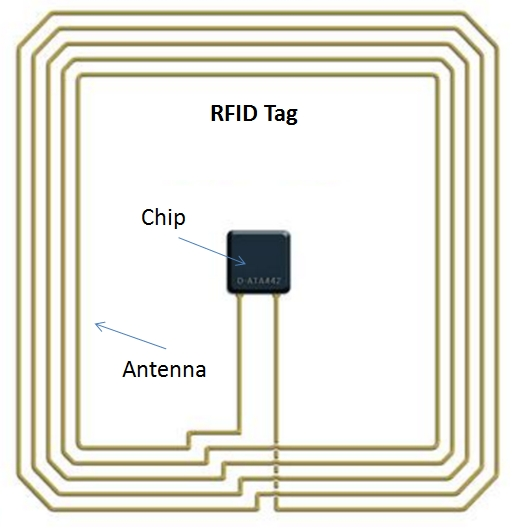
\includegraphics[width=10cm]{img/theory/NFC/RFID_tag.jpg}
	\caption{Budowa tag'a RFID. Źródło: \cite{RFID_antenna}.}
	\label{fig:image_rfid_tag}
\end{figure}

W odróżnieniu od tego, NFC (\textit{ang. \textbf{N}ear \textbf{F}ield \textbf{C}ommunication}) stanowi pełnoprawny protokół komunikacyjny. Umożliwia on wymianę długich wiadomości. Został on zbudowany na podstawie RFID i wykorzystuje jego warstwę fizyczną. Tak samo jak w RFID, w NFC można wyróżnić 2 typy urządzeń - pasywne oraz aktywne. Urządzenie pasywne nie generuje swojego własnego pola elektromagnetycznego, w przeciwieństwie do do urządzenia aktywnego, które inicjuje komunikację. Ponadto, urządzenie bierne, tak samo jak w przypadku RFID nie posiada nawet własnego źródła zasilania. Gdy znajdzie się ono w polu wygenerowanym przez urządzenie aktywne, w jego antenie wyindukuje się prąd, który jest w stanie zasilić niewielki moduł. Komunikacja zwrotna odbywa się poprzez modyfikację zużycia energii tag'a (urządzenia pasywnego) zgodnie z bitowym wzorcem, który należy wysłać. Dynamiczne zmiany parametrów zużycia powodują pewne zaburzenia wygenerowanego przez inicjator pola RF. Odczyt danych przez nie polega na odczycie zmian tego pola. Przedstawiono to na rysunku \ref{fig:image_nfc_comm}. 

\begin{figure}[H]
	\centering
	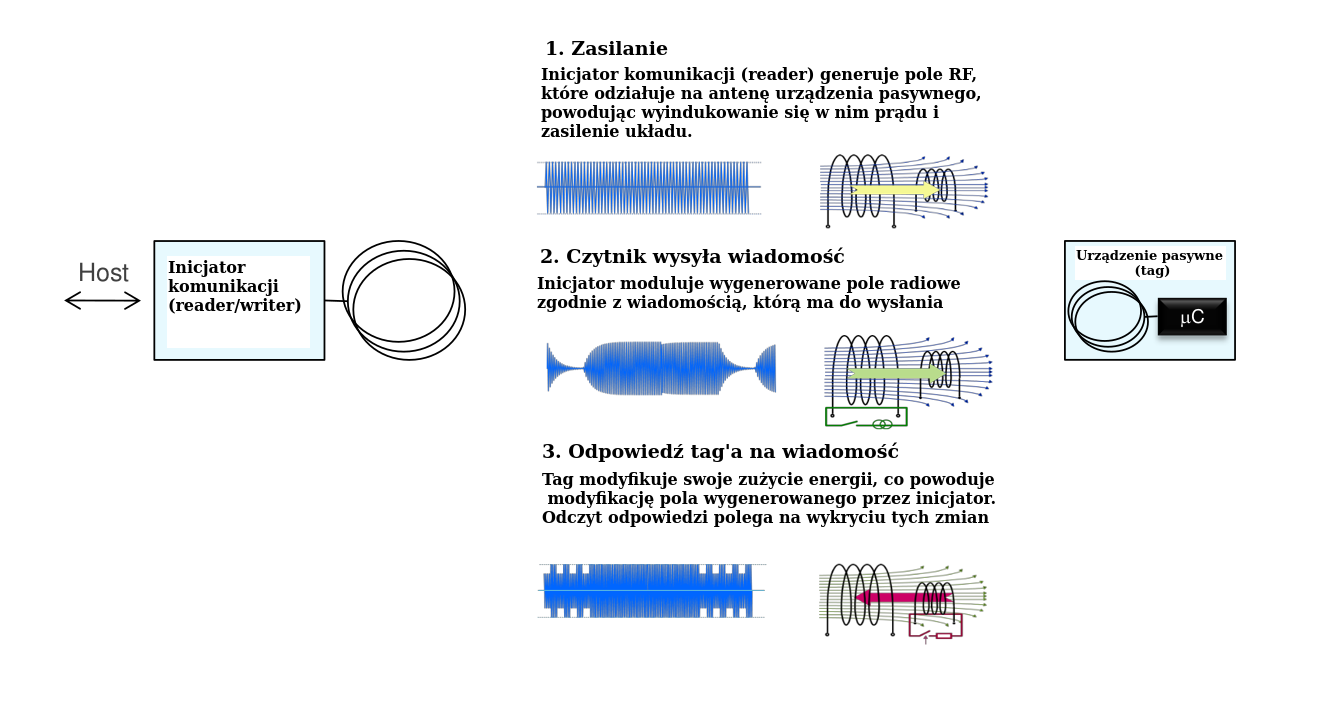
\includegraphics[width=18cm]{img/theory/NFC/NFC_communication.png}
	\caption{Zasada działania komunikacji pomiędzy urządzeniem aktywnym i pasywnym. Źródło: \cite{NFC_NXP}.}
	\label{fig:image_nfc_comm}
\end{figure}

Istnieje również możliwość komunikacji pomiędzy dwoma urządzeniami aktywnymi. Wówczas zamiast modyfikować pole wyindukowane, urządzenie odpowiada swoim własnym, wygenerowanym z energii źródła zasilania. Dzięki temu, możliwy do osiągnięcia zasięg komunikacji jest większy. 

Na tym w zasadzie podobieństwa między NFC i RFID się kończą. RFID pozwala bowiem jedynie na odpowiedź w postaci swojegu unikalnego numeru identyfikacyjnego UID (\textit{ang. \textbf{U}nique \textbf{I}dentifier \textbf{N}umber}), natomiast moduły NFC stanowią najczęściej urządzenia programowalne, pozwalające na przesłanie dowolnej wiadomości. Ponadto, kolejną różnicą jest fakt, że RFID nie posiada jednego wspólnego standardu komunikacji. Co więcej, nie posiada nawet stałej częstotliwości komunikacji, a jej wybór zależy od producenta sprzętu. Zasięg komunikacji w przypadku RFID również jest zmienny i zależny od częstotliwości sygnału. Dla wartości rzędu \linebreak 125 - 134,3 kHz wynosi ona do 30 cm (zazwyczaj około 10 cm), dla częstotliwości \linebreak 13,56 MHz - do 1,5 metra, a w przypadku 433 MHz - nawet do 500 metrów. Ta różnorodność i brak pojedynczego standardu komunikacji stała się główną przyczyną powstania protokołu NFC.

NFC pracuje na ściśle określonej częstotliwości o wartości 13,56 MHz. Zasięg komunikacji jest niewielki (rzędu 10 cm), a urządzenia mają możliwość emulowania tagów RFID, czyli zachowania się jak one gdy wykryte zostanie pole RF. Dodatkowym atutem NFC jest zdefiniowanie formatu komunikacji pomiędzy urządzeniami - NDEF (\textit{ang. \textbf{N}FC \textbf{D}ata \textbf{E}xchange \textbf{F}ormat}). Istnieją pewne dobrze znane struktury danych, możliwe do wysłania poprzez NFC.

 Są to:

\begin{itemize}
\item Wiadomości tekstowe
\item Adresy internetowe URI
\item Proste komendy
\item Podpisy cyfrowe
\end{itemize}

Organizacją zajmującą się standaryzacją i rozwijaniem NFC jest NFC Forum. Definiuje ona 4 rodzaje urządzeń pasywnych:

\begin{enumerate}
	\item Typ 1
	\begin{itemize}
		\item Bazuje na specyfikacji ISO-14443A
		\item Może być tylko do odczytu lub mieć zdolność do zapisu i odczytu
		\item Rozmiar pamięci od 96 B do 2 KB
		\item Prędkość komunikacji - 106 Kb/s
		\item Brak ochrony przed kolizją pól
	\end{itemize}
	
	\item Typ 2
	\begin{itemize}
		\item Bazuje na specyfikacji ISO-14443A
		\item Może być tylko do odczytu lub mieć zdolność do zapisu i odczytu
		\item Rozmiar pamięci od 96 B do 2 KB
		\item Prędkość komunikacji - 106 Kb/s
		\item Zapewnia mechanizm ochrony przed kolizją
	\end{itemize}
	
	\item Typ 3
	\begin{itemize}
		\item Bazuje na specyfikacji ISO-18092 i JS-X-6319-4
		\item Może być tylko do odczytu lub mieć zdolność do zapisu i odczytu
		\item Rozmiar pamięci do 1 MB
		\item Prędkość komunikacji - 212 lub 424 Kb/s
		\item Zapewnia mechanizm ochrony przed kolizją
	\end{itemize}
	\clearpage
	\item Typ 4
	\begin{itemize}
		\item Bazuje na specyfikacji ISO-18092 i JS-X-6319-4
		\item Może być tylko do odczytu lub mieć zdolność do zapisu i odczytu
		\item Rozmiar pamięci: 2, 4 lub 8 KB
		\item Prędkość komunikacji - 106, 212 lub 424 Kb/s
		\item Zapewnia mechanizm ochrony przed kolizją
	\end{itemize}
	
\end{enumerate}


